\documentclass[12pt]{article}

\usepackage[english]{babel}
\usepackage{fancyhdr}
\pagestyle{fancy}
\fancyhf{}
\lhead{Spring 2021 --- PHYS 421 Lab 1}
\rhead{Helen (Yeu) Chen}
\setlength{\parindent}{0cm}
\usepackage{makecell}
\usepackage{amsfonts}
\usepackage{longtable}
\usepackage{amsmath}
\usepackage{amssymb}
\usepackage{amsthm}
\usepackage{geometry}
\geometry{margin=1in}
\usepackage{graphicx}
\graphicspath{ {./images/} }


\fancyfoot[C]{\thepage}

\begin{document}
\textbf{Hydrogen-Deuterium Spectrum Experiment}
\bigskip

\textbf{1. \textit{Introduction}}
\smallskip


In this experiment, we used the wavelength differences between hydrogen and deuterium Balmer series to calculate the mass ratio of hydrogen and deuterium.

First, we use a monochromator to scan over the sodium spectrum at a constant rate. Since the wavelength difference between the two lines of the yellow sodium doublet is known (sodium D lines), it can be used to calculate a conversion factor between wavelength difference and time difference that depends on the scanning rate we choose. Then we measured the wavelength differences between hydrogen and deuterium Balmer series (namely: $\alpha$, $\beta$, $\gamma$, $\delta$, and $\epsilon$ lines).

Using the expression of effective mass and orbital energy difference
$$\mu = \frac{mM}{M+m}, \quad E_i -E_f \propto \mu (\frac{1}{n_f^2} - \frac{1}{n_i^2}) $$
we find that 
$$\frac{\Delta \lambda_{HD}}{\lambda_H} =  \frac{\lambda_H - \lambda_D}{\lambda_H}= \frac{1/ \mu_H - 1/ \mu_D}{1/\mu_H} = \frac{1- M_H / M_D}{1+M_H/m}$$
Since $M_H/m$ and $\lambda_H$ is known and we can measure $\Delta \lambda_{HD}$, we then can solve for the desired quantity $M_H/M_D$. To improve accuracy, we plot $\Delta \lambda_{HD}$ for all lines in the Balmer series, and fit the data to find the slop (i.e  $\frac{\Delta \lambda_{HD}}{\lambda_H}$) instead of just using one single spectral line.
\bigskip

\textbf{2. \textit{Result for the mass ratio}}
\smallskip

The data plot for $\Delta \lambda_{HD}$ with respect to hydrogen wavelength is shown below (note that the fitted line is included also)
\smallskip

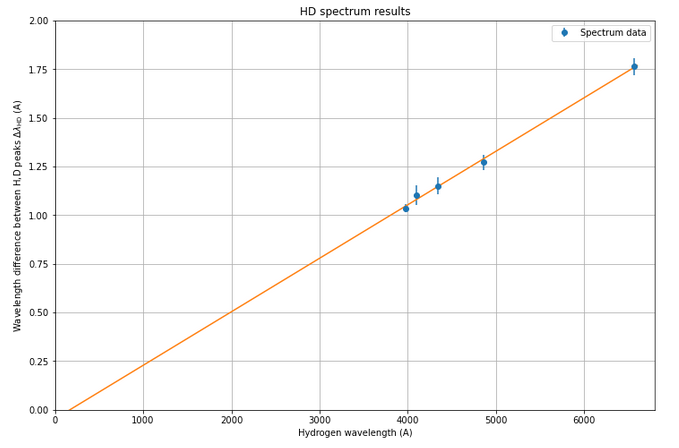
\includegraphics[width=10cm]{wavelength_difference}
\smallskip

The fitted line gives a slop of $0.000257 \pm 0.000009$. Using the equation given above, the mass ratio is: $$\frac{M_H}{M_D} = 0.49 \pm 0.02$$
The accepted value of hydrogen-deuterium mass ration is $M_H/M_D = 0.500248$, which is only about $0.01$ off from our measured value, so lies within the uncertainty ($0.02$). This concluded that our measured value agree very well with the accepted value.
\bigskip

\textbf{3. \textit{Possible error}}
\smallskip

Assume we made a mistake in measurements by pausing the wavelength scanning for 2 seconds between two sodium D lines, how would it effects our mass ratio final result?
\smallskip

First, we consider how this mistake will effect the scaling factor $K_{Na} = \frac{\Delta \lambda_{D}}{\Delta t_D}$. Since the time interval between sodium peaks is lengthened by our mistake
$$K_{Na} = \frac{\Delta \lambda_{D}}{\Delta t_D} \rightarrow \frac{\Delta \lambda_{D}}{\Delta t_D + 2}$$
The scaling factor will become smaller, namely, it is scaled by $\frac{\Delta t_D}{\Delta t +2} = 0.94026 \pm 0.00004$ (with $\Delta t_D = 31.476 \pm 0.025$ from our analysis).

Since we calculate $\Delta \lambda_{HD}$ values using $ K_{Na}$ as follow
$$ \Delta \lambda_{HD} = K_{Na} \Delta t_{HD}$$
the new $\Delta \lambda_{HD}$ will also be scaled by the same amount (i.e $\Delta \lambda_{HD} \rightarrow 0.94026 \Delta \lambda_{HD}$). So the slope ($\frac{\Delta \lambda_{HD}}{\lambda_H}$) will also decrease by a factor of $0.94026$. Solving for the mass ratio in the equation on the first page, with the known value $M_H / m = 1836.15$, we get 
$$\frac{M_H}{M_D} = 1- 1837.15 \times \frac{\Delta \lambda_{HD}}{\lambda_H}$$
this means that a 0.94026 decrease in slope will result in a new mass ratio of $0.525 \pm 0.015$ (original slope is $0.000275 \pm 0.000009$, detailed calculation is done in the analysis notebook). So, by taking the ratio of the "correct mass ratio" and the "incorrect mass ratio" 
$$\frac{(M_H/M_D)_{incorrect}}{(M_H/M_D)_{correct}} = \frac{0.525 \pm 0.015}{0.49 \pm 0.02} = 1.061 \pm 0.004$$
So the mistake we made causes us to measure a mass ratio that is $106.1 \%$ of the mass ratio without making the mistake.  

\end{document}